% diese Datei enthaelt den eigentlichen Vortrag, siehe Handbuch zur Latex "Beamer" Klasse

\mode<presentation>
{

  % Theme fuer das Rechen- und Kommunikationszentrum der RWTH Aachen
  \usetheme{RWTHRZ}

  %\usecolortheme{lily}
  %\usecolortheme{seahorse}

}


% diverse weitere Pakete
\usepackage[german]{babel}
\usepackage[latin1]{inputenc}
\usepackage{times}
\usepackage[T1]{fontenc}
\usepackage{graphicx}


\title[Vorstellung DHCPAdmin]           % kurzer Titel, eventuell nicht noetig
{Kurzvorstellung DHCP Administration}   % langer Titel

% \subtitle{foobar}                     % Untertitel, wenn es einen gibt

\author[Hektor, Neumann]{}              % Autor(en)

\date[\today]                           % Datum oder Konferenz, kurz
{\today}                                % Datum oder Konferenz, lang


% Folgendes sollte gel�scht werden, wenn man nicht am Anfang jedes
% Unterabschnitts die Gliederung nochmal sehen m�chte.
%\AtBeginSubsection[]
%{
%  \begin{frame}<beamer>
%    \frametitle{Gliederung}
%    \tableofcontents[currentsection,currentsubsection]
%  \end{frame}
%}


\begin{document}

\begin{frame}
  \titlepage
\end{frame}

\begin{frame}
  \frametitle{"Ubersicht}
  \tableofcontents
  % Die Option [pausesections] k�nnte n�tzlich sein.
\end{frame}



% Einen Vortrag zu strukturieren ist nicht immer einfach. Die
% nachfolgende Struktur kann unangemessen sein. Hier ein paar Regeln,
% die f�r diese L�sungsvorlage gelten:

% - Es sollte genau zwei oder drei Abschnitte geben (neben der
%   Zusammenfassung).
% - *H�chstens* drei Unterabschnitte pro Abschnitt.
% - Pro Rahmen sollte man zwischen 30s und 2min reden. Es sollte also
%   15 bis 30 Rahmen geben.

% - Konferenzteilnehmer wissen oft wenig von der Materie des
%   Vortrags. Deshalb: vereinfachen!
% - In 20 Minuten ist es schon schwer genug, die Hauptbotschaft zu
%   vermitteln. Deshalb sollten Details ausgelassen werden, selbst
%   wenn dies zu Ungenauigkeiten oder Halbwahrheiten f�hrt.
% - Falls man Details wegl�sst, die eigentlich wichtig f�r einen
%   Beweis/Implementation sind, so sagt man dies einmal n�chtern. Alle
%   werden damit gl�cklich sein.

\section{Motivation}

\subsection{Das Problem}

\begin{frame}
    \frametitle{Das Problem}

    \begin{itemize}
        \item Eintragen und "Andern von MAC-/IP-Adressen nur durch das NOC m"oglich.
        \item Kein direktes Feedback f"ur den Anwender (''Mail schicken und warten...'').
    \end{itemize}
\end{frame}

\subsection{Die L"osungsidee}

\begin{frame}
    \frametitle{Die L"osungsidee}

    Programmieren einer eigenen Web-Anwendung, Features:

    \begin{itemize}
        \item Authentifizierung durch TIM (via Radius).
        \item Ausreichende Validierung von Benutzereingaben.
        \item Direktes Einspielen aktualisierter Daten m"oglich.
        \item Einfache Administration.
    \end{itemize}
\end{frame}

\section{Implementation}

\subsection{Verwendetes Backend und Framework}

\begin{frame}
    \frametitle{Backend und Framework}

    \begin{itemize}
        \item Ruby on Rails als Framework.
        \item PostgreSQL als Datenbank.
        \item Apache als Webserver.
    \end{itemize}
\end{frame}

\begin{frame}
    \frametitle{Daten"ubermittlung}

    Daten"ubermittlung an die Cisco-Switches:

    \begin{itemize}
        \item Generieren einer Cisco-DHCP Configdatei.
        \item Direkt via Telnet (wenn entsprechend konfiguriert).
    \end{itemize}
\end{frame}

\subsection{Benutzeroberfl"ache}

\begin{frame}
    \frametitle{Benutzeroberfl"ache}

    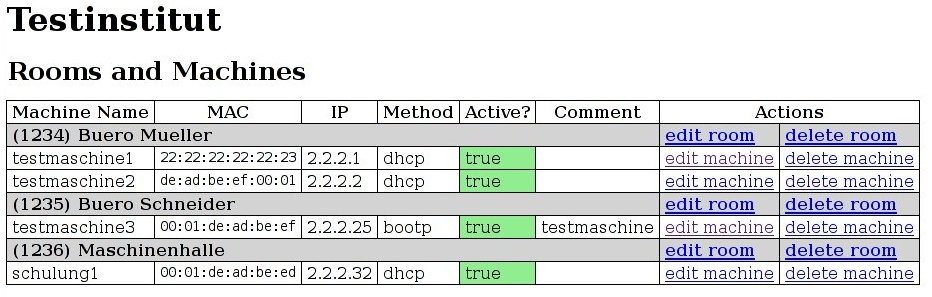
\includegraphics[width=11cm]{gui1}

    \begin{itemize}
        \item "Ubersichtlich.
        \item Unterst"utzt Organisationseinheit ,,R"aume''
        \item Einzelne Eintr"age k"onnen zeitweise deaktiviert werden.
    \end{itemize}

\end{frame}

\begin{frame}
    \frametitle{Validierung von Benutzereingaben}

    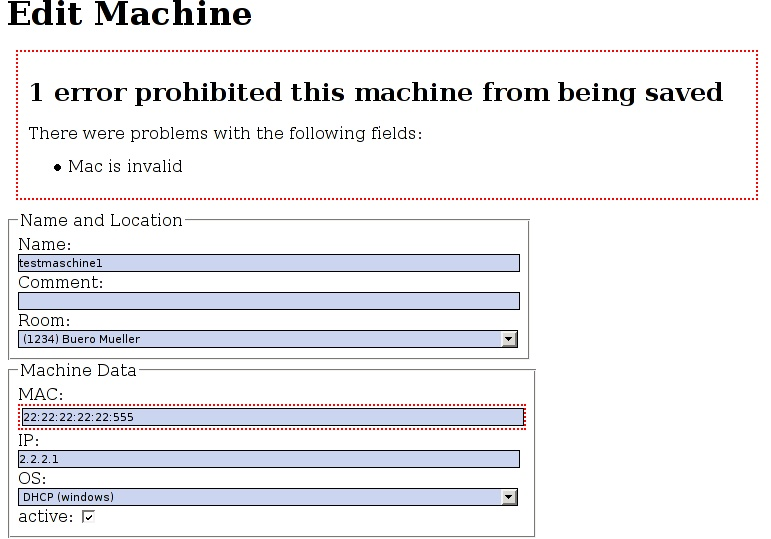
\includegraphics[height=7cm]{gui2}
\end{frame}

\begin{frame}
    \frametitle{Ausblick: DNS-Administration?}

    M"oglichkeit: DNS-Administration integrieren.
    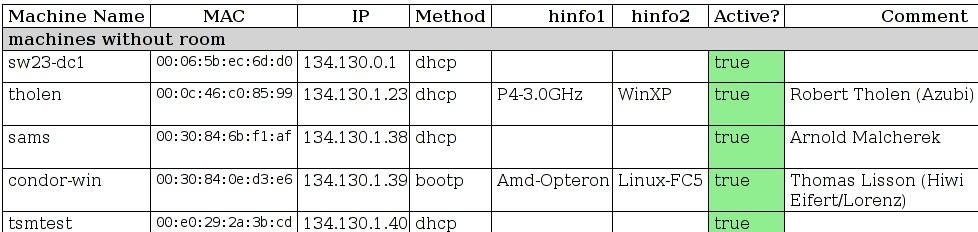
\includegraphics[width=11cm]{gui3}
\end{frame}

\begin{frame}
    \frametitle{Validierung von Benutzereingaben}

    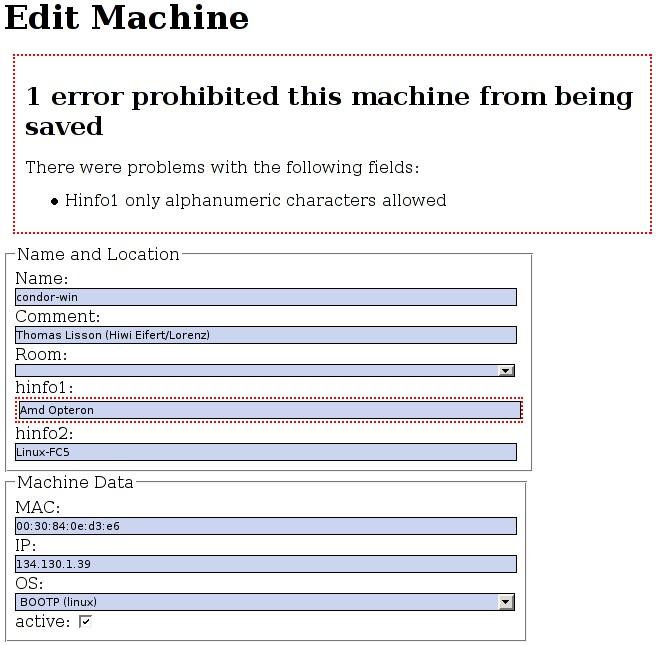
\includegraphics[height=7cm]{gui4}
\end{frame}

\begin{frame}[fragile]
    \frametitle{DNS Zonefile generieren}

    \scriptsize
    \begin{verbatim}
tholen      IN      A  134.130.1.23    ; Robert Tholen (Azubi)
            IN  HINFO  "P4-3.0GHz"     "WinXP"
sams        IN      A  134.130.1.38    ; Arnold Malcherek
condor-win  IN      A  134.130.1.39    ; Thomas Lisson (Hiwi Eifert/Lorenz)
            IN  HINFO  "Amd-Opteron-1GHz"      "Linux-FC5"
    \end{verbatim}
\end{frame}

\section{Zusammenfassung/Feedback}

\begin{frame}
    \frametitle{Zusammenfassung und Feedback}

    \begin{itemize}
    \item Webbasiertes datenbankgest�tztes Interface zur delegierten Administration von DHCP-Daten.
    \item Entlastung des NOC.
    \item Schnelle Aktivierung von �nderungen durch ''Selfservice''.
    \item Benutzerfeedback durchweg sehr positiv.
    \end{itemize}

    Zukunft: Selfservice f�r DNS-Daten?

\end{frame}

\end{document}
